\documentclass[a4paper,12pt]{article}
\usepackage[utf8]{inputenc}
\usepackage[T2A]{fontenc}
\usepackage[russian]{babel}
\usepackage{amsmath,amssymb}
\usepackage{graphicx}
\usepackage{caption}
\usepackage{listings}
\usepackage{hyperref}
\usepackage{seqsplit} % Для переноса длинных чисел




\lstset{
    basicstyle=\ttfamily\small,
    breaklines=true,
    frame=single,
    captionpos=b,
    numbers=left,
    numberstyle=\tiny,
    language=Python
}

\begin{document}

\section*{Отчёт по лабораторной работе 2}

\bigskip

\textbf{Студент:} Кочкожаров Иван Вячеславович

\noindent
\textbf{Группа:} \underline{М8О-308Б-22}

\bigskip

\noindent
\textbf{Цель работы:} получить вариант на основе хеш-функции ГОСТ Р 34.11-2012 (Стрибог) и выполнить нетривиальное разложение чисел $a$ и $b$ на простые множители.

\section{Постановка задачи}
На вход хеш-функции Стрибог подаётся строка с ФИО автора. Из выходного 256‑битного хеша берутся младшие 8 бит — число от 0 до 255, которое и служит номером варианта. Для данного варианта необходимо:
\begin{enumerate}
    \item Извлечь значения $a$ и $b$ из списка вариантов.
    \item Разложить каждое из чисел $a$ и $b$ на нетривиальные сомножители.
\end{enumerate}
\newpage

\section{Получение номера варианта}

\begin{lstlisting}[caption={Функция для вычисления варианта по ФИО}]
from gostcrypto import gosthash

def get_variant_number(full_name: str):
    data_bytes = full_name.encode('utf-8')
    hash_256 = gosthash.new('streebog256', data=data_bytes)
    digest = hash_256.digest()
    return digest[-1]
\end{lstlisting}

\begin{figure}[h!]
    \centering
    % Вставьте здесь ваш скриншот выбора варианта
    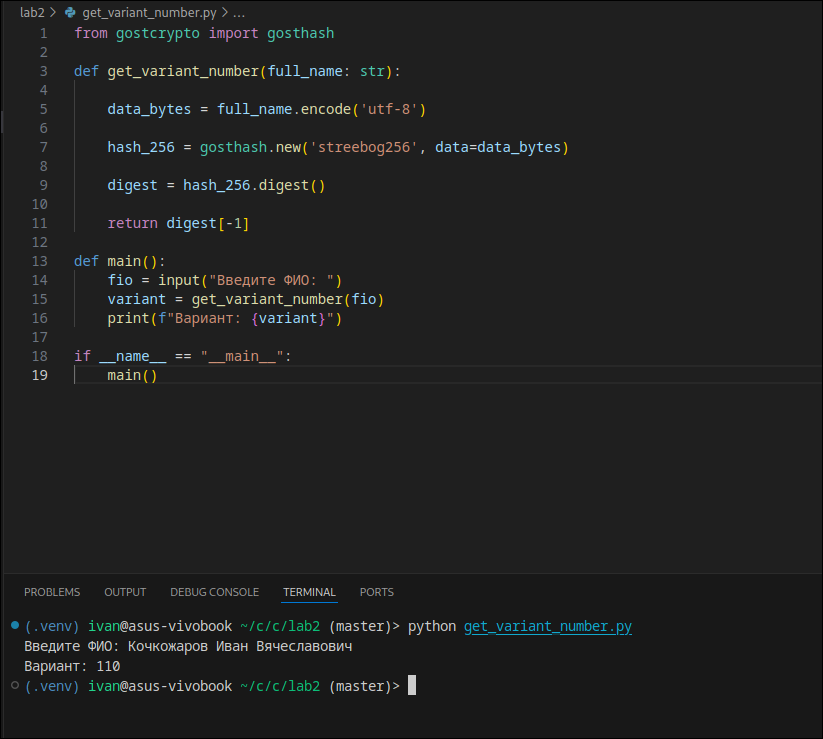
\includegraphics[width=1\textwidth]{screenshot.png}
    \caption{Номер варианта, полученный из ФИО}
    \label{fig:variant}
\end{figure}

\noindent
Запустив скрипт с ФИО «\textit{Кочкожаров Иван Вячеславович}», получили:



\medskip
\noindent
\textbf{Результат:} номер варианта: 110.

a = \seqsplit{96549329211410878220407731243138541789894262114809366396824543095582747523721}

b = \seqsplit{32317006071311007300714876688669951960444102669715484032130345427524655138867890893197201411522913463688717960921898019494119559150490921095088153368755819279948894891352978038724364814666828075403374368623252601199573103732364197539194324809397600124011761205890421945836628563695877139401393419600972620930627469732652285701750217853272073677807696706525660813610654888881988572347249424515008349686030605536267873810768793941519437795740337005159565713224668295133294397929491874554881716226163300019068770229099948764818609237849953239277955372804162008595934215621479331566395118297110850271069157386069736822127}

\section{Разбор алгоритма факторизации}

\subsection{Разложение числа \(a\)}
Для числа \(a\) классический подход через \texttt{sympy.factorint} даёт ответ за малое время:
\begin{lstlisting}[caption={Разложение \(a\) с помощью Sympy}]
import re
from PyPDF2 import PdfReader
from sympy import factorint

factors_a = factorint(a)
print("Factor a:")
print(" * ".join(str(p) for p, exp in factors_a.items() for _ in range(exp)))
\end{lstlisting}

\noindent
\textbf{Результат:} 
a = 15381195539196285749 $\times$ \seqsplit{6277101735386680763835789423207666416102355444464034513029}

\subsection{«Трудное» разложение числа \(b\)}
Число \(b\) из условия слишком велико для прямого перебора. Поэтому была применена следующая идея:

\begin{itemize}
    \item Было предположено, что каждое \(b_i\) состоит ровно из двух простых сомножителей.
    \item Для каждого другого варианта \(b_j\) вычисляется \(\gcd(b, b_j)\).
    \item Если \(\gcd(b, b_j)\) — простое число \(p\) и \(b/p\) - простое число, то мы нашли два множителя.
\end{itemize}

\noindent
Соответственно, для автоматизации перебора был написан скрипт:

\begin{lstlisting}[caption={Поиск простого делителя через НОД}]
from math import gcd
from sympy import isprime
#bs - all b from other variants
for other_b in bs:
    d = gcd(b, other_b)
    if isprime(d):
        p = d
        q = b // d
        if isprime(q):
            print("b = {} * {}".format(p, q))
            break
\end{lstlisting}

\noindent
Предроложение о числах оказалось верным, и таки образом удалось быстро найти нетривиальное разложение числа \(b\).

\medskip
\noindent
\textbf{Результат:}

b = \seqsplit{2410312426921032588580116606028314112912093247945688951359675039065257391591803200669085024107346049663448766280888004787862416978794958324969612987890774651455213339381625224770782077917681499676845543137387820057597345857904599109461387122099507964997815641342300677629473355281617428411794163967785870370368969109221591943054232011562758450080579587850900993714892283476646631181515063804873375182260506246992837898705971012525843324401232986857004760609160377} $\times$ \seqsplit{13407807929942597099574024998205846127479365820592393377723561443721764030073546976801874298166903427690031858186486050853753882811946569946433649413627751}


\section{Выводы}
\begin{enumerate}
    \item Метод вычисления варианта по хеш-функции Стрибог продемонстрирован и реализован в виде скрипта на Python.
    \item Число \(a\) было факторизовано стандартными средствами Sympy.
    \item Для числа \(b\) найден эффективный приём через поиск общих делителей с другими вариантами, для перебора был применен парсинг pdf.
    \item В отчёте приведены алгоритмы и результаты разложения.
\end{enumerate}

\bigskip
\noindent
\textbf{Приложение. Исходный код}
\begin{lstlisting}[caption={get\_variant\_number.py}]
from gostcrypto import gosthash

def get_variant_number(full_name: str):

    data_bytes = full_name.encode('utf-8')

    hash_256 = gosthash.new('streebog256', data=data_bytes)

    digest = hash_256.digest()

    return digest[-1]

def main():
    fio = input("Введите ФИО: ")
    variant = get_variant_number(fio)
    print(f"Вариант: {variant}")    

if __name__ == "__main__":
    main()
\end{lstlisting}

\begin{lstlisting}[caption={main.py}]
import re
from sympy import factorint, isprime
from math import gcd
from PyPDF2 import PdfReader
from get_variant_number import get_variant_number


def parse_pdf(pdf_path):
    reader = PdfReader(pdf_path)
    full_text = ""
    for page in reader.pages:
        full_text += page.extract_text()
    
    text_clean = re.sub(r"\s+", "", full_text)
    
    pattern = r"a\[([0-9]+)\]=([0-9]+).*?b\[\1\]=([0-9]+)"
    
    matches = re.findall(pattern, text_clean, re.DOTALL)
    pairs = [(int(a), int(b)) for _, a, b in matches]
    return pairs

def main():
    pdf_path = "Лабораторная 2.pdf"
    full_name = "Кочкожаров Иван Вячеславович"
    variant_number = get_variant_number(full_name)
    print(f"ФИО: {full_name}")
    print(f"Вариант: {variant_number}")
    pairs = parse_pdf(pdf_path)
    a = pairs[variant_number][0]
    b = pairs[variant_number][1]
    print(f"a = {a}")
    print(f"b = {b}")

    bs = [b for _, b in pairs]
    bs.pop(variant_number)
    factors_b=[]
    for other_b in bs:
        divisor1 = gcd(b, other_b)
        if (isprime(divisor1)):
            divisor2 = b // divisor1
            if (isprime(divisor2)):
                factors_b.append(divisor1)
                factors_b.append(divisor2)
                break
    print("Разложение b:")
    print(*factors_b, sep=' * ')

    print("Разложение a: ")
    factors_a_dict = factorint(a)
    factors_a = [key for key, count in factors_a_dict.items() for _ in range(count)]
    print(*factors_a, sep=' * ')

if __name__ == "__main__":
    main()
\end{lstlisting}

\end{document}
